%%% result.tex 
%% displays experimental setup, and description of matrices 
We performed a series of experiments to test robustness and overhead of our algorithm described in~\refsec{sec:connected}. 

%ODED - this subsection should be part of the experimental setup/
\subsection{Fault Injection Methodology}
Since memory accesses are most performance critical part in~\sv computation, we inject faults in memory access pattern. There are two main memory accesses in~\sv iteration: traversing adjacency list for each vertex; and 
accessing $CC$ array for each vertex in adjacency list. 


%ODED - in our meeting yesterday you stated that f was not a rate (between 0 and 1) rather it represented the actual number of errors.  Here is seems that it is rate.  
In the first case, before each~\sv sweep, we randomly select $f|E|$ edges, where $f$ is fault-rate. Let $e=(v,u)$ be  one of the selected edges. When we encounter $e$ while traversing adjacency list of $v$, we flip one of the bits of $u$---the vertex which $e$ is pointing---randomly. 
Therefore, due to the fault, $v$ will visit flipped vertex $\hat{u}$, instead of accessing $u$. 

In the second case, we will again choose another set of $f|E|$ edges. Let $e=(v,u)$ be  one of the selected edges. When we encounter $e$ while traversing adjacency list of $v$, we flip one of the bits of $CC[u]$.
Therefore, due to the fault, $v$ will visit the correct vertex, however, it see incorrect value of  $CC[u]$.
It should be noted that $CC[u]$ will be accessed multiple times in a~\sv iteration, and we assume that 
all accesses to $CC[u]$ in an iteration are independent. In other words, if $CC[u]$ is accesses while visiting 
vertex $v_{1},\ v_{2}$, and if $CC[u]$ is corrupted while visiting $v_{1}$, then $CC[u]$ may or may not be corrupted when it is accessed while visiting $v_{2}$.


\subsection{Experimental Setup}


%ODED - the term "matrix" should never appear in the paper. We should only use the term "network" or "graph"
% type of matrices 
\paragraph{Test Graphs}
The graphs used in our tests are listed in~\reftab{tab:graphs}. 
These graphs are taken from the 10th Dimacs Implementation Challenge~\cite{Bader-dimacs-graph2014}, come from various real and synthetic applications. 
\begin{table*}[]
\centering
\caption{List of matrices used for experimentation}
\label{tab:matrix}
\begin{tabular}{llll}
Matrix Name              & Source                      & \#Vertices & \#Edges  \\
astro-ph                 & collaboration network       & 16706      & 242502   \\
audikw1                  & UF Sparse Matrix Collection & 943695     & 77651847 \\
caidaRouterLevel         & Clustering                  & 192244     & 1218132  \\
cnr-2000                 &                             & 325557     & 2738969  \\
coAuthorsDBLP            &                             & 299067     & 977676   \\
coPapersDBLP             &                             & 540486     & 15245729 \\
cond-mat-2005            &                             & 40421      & 175691   \\
delaunay\_n18            &                             & 262144     & 786396   \\
er-fact1.5-scale20       &                             & 1048576    & 10904496 \\
G\_n\_pin\_pout          &                             & 100000     & 501198   \\
kron\_g500-simple-logn18 &                             & 262144     & 10582686 \\
ldoor                    &                             & 952203     & 22785136 \\
preferentialAttachment   &                             & 100000     & 499985   \\
rgg\_n\_2\_18\_s0        &                             & 262144     & 1547283 
\end{tabular}
\end{table*}

\paragraph{Testbed}
\begin{table}[]
\centering
\caption{Testbeds used for performance evaluation.}
\label{tab:sys_info}
\begin{tabular}{ll}
Prop                 & SNB20c       \\
Sockets$\times$Cores & 2$\times$8   \\
Clock Rate           & 2.4GHz       \\
DRAM capacity        & 128GB        \\
DRAM Bandwidth       & 72GB/s      
\end{tabular}
\end{table}
We prototyped baseline and fault tolerant implementation using $C$ language. 
We used the Intel C Compiler (ICC 15.0.0), with highest level of
 optimization $-O3$ to compile our benchmarks.
%ODED - instead of using a table for this system, I would probably just put the properties in text.
%ODED - be specific on the type of processor being Intel Xeon XYZW
We ran all our experiments on SNB16c, key properties of the systems are listed in~\reftab{tab:sys_info}


\subsection{Convergence in presence of faults}

\begin{figure}[tbp]
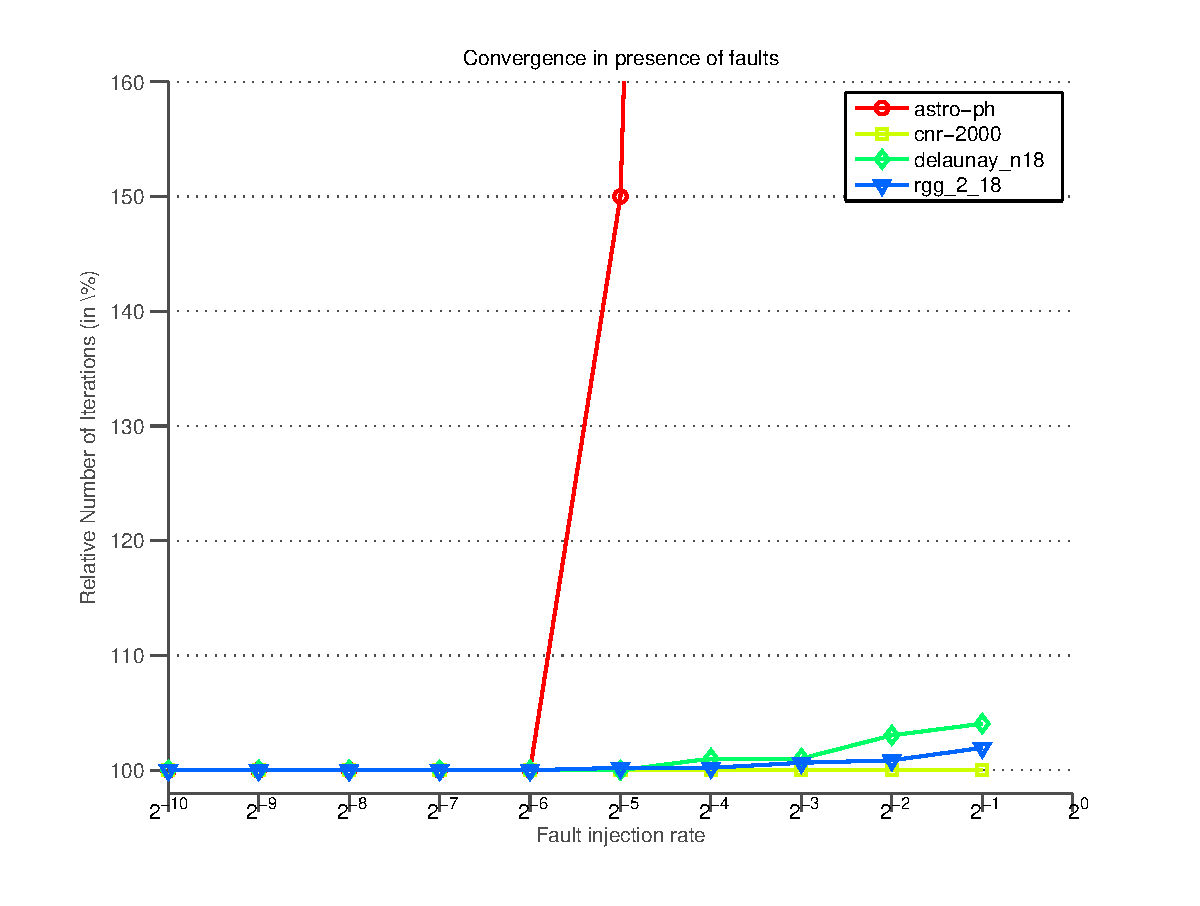
\includegraphics[width=.5\textwidth]{plots/plot_conv.eps}
\caption{\label{fig:con-plot} 
\small Comparison of model-driven work partitioning scheme to
two static work partitioning scheme}
\end{figure}

First, we try to understand the convergence property of~\sv algorithm 
in presence of faults. 
Recall that in the worst case, an \emph{acceptable} fault that is not detected by~\refalg{alg:FTSV_ALG}, may delay the convergence by one iteration. On the other hand, one additional iteration means additional faults, which may necessitate an additional iteration for convergence. 
Thus, it is expected that with increasing fault rate, convergence might slow down. To understand practicality of our algorithm, it becomes essential to understand such slow down in convergence.  

% what do we do
In~\reffig{fig:con-plot}, we show the convergence of \sv~algorithm in presence of faults for four graphs. We vary the fault rate from $2^-{10} \times |E|$ bit flips in every~{\sv}~ iteration to $2^-{1} \times |E|$ bit flips. Note that this fault injection rate is extremely high and, we do so to stress test the proposed algorithm.

%what do we observe
In~\reffig{fig:con-plot}, we observe that for all practical fault rates($<2^{-6}|E|$) , algorithm converges without any additional iteration.
Additionally, except~\graphname{astro-ph}, all other graphs converge to correct solution within 5\% additional iteration at the highest fault rate. As such, we conclude that our proposed algorithm can withstand high fault rates, with minimal additional iteration overhead.   

% why do we observe that
The difference in behavior between graph~\graphname{astro-ph}, and other graphs is due to two reasons. First, the graph~\graphname{astro-ph} has  the smallest diameter all four test cases, and it only takes 10 iterations in fault free case to converge. If a fault that might cause an additional iteration occurs, it provides fewer opportunity to be corrected in later iterations. Secondly, ...

\subsection{Overhead of fault detection and correction}

\begin{figure}[ht]
\includegraphics[width=.6\textwidth]{plots/plot_zero_overhead.eps}
\caption{\label{fig:zero-oh-plot} 
\small Comparison of model-driven work partitioning scheme to
two static work partitioning scheme}
\end{figure}

\paragraph{Overhead with increasing Faults}


%% compare it with double modular redundancy 
In addition to extra iteration to converge, extra computation that goes in 
fault detection  and correction can be also a source of significant overhead. 
We analyze overhead of fault detection and correction in two parts.
 First, we evaluate the overhead of algorithm \ftsv when no faults are injected.
  Then, we evaluate how overhead of proposed algorithm behaves at different fault rates. 

\paragraph{Zero-Overhead} Zero-overhead denotes the overhead of the algorithm 
in absence of any injected faults. In this case, all the additional computation
 goes into fault detection. We compare the zero-overhead of~\refalg{alg:FTSV_ALG}, with 
 fault free execution of~\refalg{alg:SV_ALG}. 

 %
 In~\reffig{fig:zero-oh-plot}, we show the \emph{relative} zero-overhead of~\refalg{alg:FTSV_ALG} 
 different test graphs. In all the test cases, zero-overhead remains smaller than 25\%. 
 In the graphs with smaller $|E|/|V|$ ratio, for instance~\graphname{citationCiteseer} ($|E|/|V|=4.3$),
 \graphname{coAuthorsDBLP} (3.3), \graphname{rgg\_n\_2\_18\_s0} (5.9), have large zero-overhead. On the other hand graphs with large $|E|/|V|$ ratio such as \graphname{kron\_g500-simple-logn18} ($|E|/|V|=40$), we observe small zero-overhead. This variation of zero-overhead with $|E|/|V|$ ratio, us expected as asymptomatic complexity of fault detection in an ~\ftsv iteration is $\mathcal{O}(V)$, while cost of an ~\sv iteration is $\mathcal{O}(|V|+|E|)$.  

\paragraph{Overhead of~\ftsv in presence of faults}

\begin{figure}[ht]
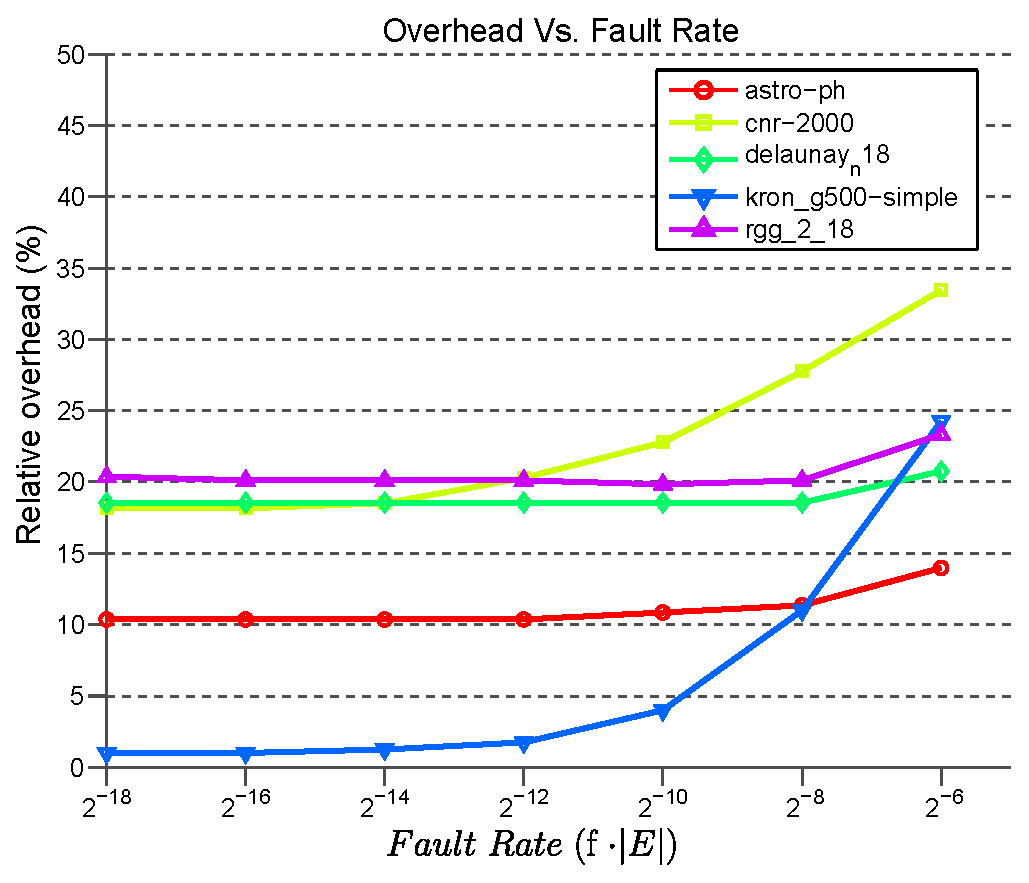
\includegraphics[width=.5\textwidth]{plots/plot_overhead_fault.eps}
\caption{\label{fig:oh-plot} 
\small Comparison of model-driven work partitioning scheme to
two static work partitioning scheme}
\end{figure}

We evaluated overhead of~\ftsv in presence of faults to understand scalability of the proposed algorithm 
with increasing fault rates. To do so, we vary fault rates from $2^-{18}|E|$ to $2^-{6}|E|$ distinct bit
flips in every iteration for all test graphs. In~\reffig{fig:oh-plot}, we show the the relative overhead 
of ~\ftsv algorithm with respect to increasing fault rates for four matrices.
We expect that overhead will increase linearly with increasing fault rates.
For all the four matrices, overhead of fault detection is small for fault rates upto $2^{-10}|E|$ bit flips 
in every iteration. Beyond $2^{-10}|E|$, we see overhead increasing slowly, however increase in all the cases 
is sub-linear. 
This is due to many graphs considered in our study follows power law distribution of for degree of vertices, thus
these graphs have very high number of vertices with very small degrees, thus correction 
for large number of vertices are $\mathcal{O}(1)$ operations. 
Among all the graphs tested, the graph \graphname{kron\_g500-simple-logn18} showed steepest increase in overhead with increasing
 fault rates. The graph \graphname{kron\_g500-simple-logn18} is a random Kronecker geometric graph and
  has very uniform distribution of degree among vertices, and 
  thus with fault rate, correction cost shows  linear increase. 
In all cases even in the highest fault rates considered in the paper, net overhead of \ftsv were smaller than 35\%.
 In contrast to that, naive redundency based fault tolerance algorithm will have overhead of more than 100\%. 
 Thus, we see that \ftsv can tolerate efficiently withstand high fault rates.  





